\subsection{ANGULAR SECTORS}

Given two distinct closed rays \(\Delta_{1}, \Delta_{2}\) with origin \(o\) , let \(x\) be the principal measure of the angle \((\widehat{\Delta_{1}, \Delta_{2}})\) (relative to a base \(a\) , chosen once and for all). The union of the closed (resp. open) rays \(\Delta\) with origin \(o\) which are such that the principal measure \(y\) of the angle \((\widehat{\Delta_{1}, \Delta})\) satisfies \(o \leqslant y \leqslant x\) (resp. \(o < y < x\) ) is the closed (resp. open) angular sector \(S\) with origin \(\Delta_{1}\) and extremity \(\Delta_{2}\) , as defined in algebra. For by means of a rotation we can always reduce to the case where \(S\) does not contain the ray through the point \(-1\) . If \(\alpha\) and \(\beta\) are then the angles which \(\Delta_{1}\) and \(\Delta_{2}\) respectively make with the positive real semi-axis, then the closed angular sector \(S\) is the union of the closed half-lines \(\Delta\) which make an angle \(\theta\) with the positive real semi-axis such that \(\tan \frac{1}{2} \alpha \leqslant \tan \frac{1}{2} \theta \leqslant \tan \frac{1}{2} \beta\) . Now if \(u, v, t\) are the measures of \(\alpha, \beta, \theta\) respectively which lie in the interval \([- \frac{1}{2} a, + \frac{1}{2} a[\) , these inequalities are equivalent to \(\tan_{a} \frac{1}{2} u \leqslant \tan_{a} \frac{1}{2} t \leqslant \tan_{a} \frac{1}{2} v\) ; and since \(\tan_{a} x\) is an increasing function in the interval \([- \frac{1}{4} a, + \frac{1}{4} a[\) , they are also equivalent to \(u \leqslant t \leqslant v\) , or to \(o \leqslant t - u \leqslant v - u\) ; since \(x = v - u\) , \(y = t - u\) , the result is proved for closed angular sectors, and the proof for open ones is similar.

A closed angular sector is a closed set in \(R^{2}\) , and the open angular sector with the same origin and the same extremity is its interior in \(R^{2}\) (Chapter VI, § 2, no. 3, Proposition 3). The angle \((\widehat{\Delta_1, \Delta_2})\) , with principal measure \(x\) , is called the angle of the sector S; S is said to be salient if \(x < \frac{1}{2} a\) , flat (or a closed half-plane) if \(x = \frac{1}{2} a\) ; re-entrant if \(x > \frac{1}{2} a\) . A salient angular sector is acute if \(x < \frac{1}{4} a\) , right if \(x = \frac{1}{4} a\) , obtuse if \(x > \frac{1}{4} a\) . The bisector of the sector S is the ray \(\Delta\) which makes an angle \(y = \frac{1}{2} x\) with \(\Delta_1\) .

\pandocbounded{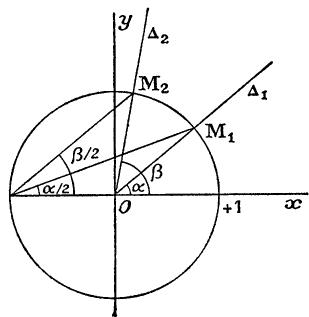
\includegraphics[keepaspectratio]{images/part001_1c4c55ab.jpg}}\\
Figure 10.

Two distinct closed rays \(\Delta_{1}, \Delta_{2}\) determine two closed angular sectors; their union is the real plane \(R^{2}\) , and their intersection is \(\Delta_{1} \cup \Delta_{2}\) .

